\documentclass[12pt,a4paper]{article}

\usepackage[utf8]{inputenc}
\usepackage[T1]{fontenc}

\usepackage[top=2.5cm,bottom=2.5cm,left=2.8cm,right=2.8cm]{geometry}
\usepackage[dvipsnames,svgnames,x11names]{xcolor}

\definecolor{androidgreen}{HTML}{3DDC84}
\definecolor{darkbg}{HTML}{1A0A2E}
\definecolor{lightgray}{HTML}{F5F5F5}
\definecolor{codebg}{HTML}{F0F8F4}
\definecolor{commentgreen}{HTML}{2E7D32}
\definecolor{keywordblue}{HTML}{1565C0}
\definecolor{stringorange}{HTML}{E65100}
\definecolor{linenumgray}{HTML}{9E9E9E}
\definecolor{infobg}{HTML}{E8F5E9}
\definecolor{warnbg}{HTML}{FFF8E1}
\definecolor{warnframe}{HTML}{F9A825}

\usepackage{graphicx}
\usepackage{tikz}
\usetikzlibrary{shapes.geometric,arrows.meta,positioning,calc,fit,backgrounds}
\usepackage{tcolorbox}
\tcbuselibrary{skins,breakable}

\usepackage{listings}
\lstdefinestyle{javaStyle}{
  backgroundcolor=\color{codebg},
  commentstyle=\color{commentgreen}\itshape,
  keywordstyle=\color{keywordblue}\bfseries,
  stringstyle=\color{stringorange},
  numberstyle=\tiny\color{linenumgray},
  basicstyle=\ttfamily\footnotesize,
  breaklines=true,
  keepspaces=true,
  numbers=left,
  numbersep=8pt,
  showstringspaces=false,
  tabsize=2,
  frame=none,
  xleftmargin=18pt,
  aboveskip=0pt,
  belowskip=0pt,
}
\lstset{style=javaStyle}

\usepackage{booktabs}
\usepackage{tabularx}
\usepackage{colortbl}
\usepackage{float}
\usepackage{titlesec}
\usepackage{parskip}
\usepackage[colorlinks=true,linkcolor=darkbg,urlcolor=androidgreen]{hyperref}
\usepackage{fancyhdr}

\pagestyle{fancy}
\fancyhf{}
\renewcommand{\headrulewidth}{0pt}
\fancyhead[L]{\small\color{gray}\texttt{Clash Royale Social API}}
\fancyhead[R]{\small\color{gray}Parcial 2 --- Mayo 2026}
\fancyfoot[C]{\small\color{gray}\thepage}

\titleformat{\section}
  {\color{darkbg}\large\bfseries}{}
  {0em}
  {\colorbox{androidgreen}{\color{white}\makebox[0.5cm][c]{\thesection}}\quad}
  [\vspace{-0.3em}\textcolor{androidgreen}{\rule{\linewidth}{1.5pt}}]

\titleformat{\subsection}
  {\color{darkbg}\normalsize\bfseries}
  {\color{androidgreen}\thesubsection\;}{0em}{}

\titleformat{\subsubsection}
  {\color{darkbg}\small\bfseries\itshape}{}{0em}{}

\newtcolorbox{patternbox}[2][]{
  enhanced, breakable,
  colback=infobg, colframe=androidgreen,
  fonttitle=\bfseries\small, title=#2,
  arc=4pt, boxrule=1.5pt,
  left=8pt, right=8pt, top=6pt, bottom=6pt, #1
}

\newtcolorbox{warnbox}[1]{
  enhanced, colback=warnbg, colframe=warnframe,
  fonttitle=\bfseries\small, title=#1,
  arc=4pt, boxrule=1.5pt,
  left=8pt, right=8pt, top=6pt, bottom=6pt,
}

\newtcolorbox{infobox}{
  enhanced, colback=infobg, colframe=androidgreen,
  arc=4pt, boxrule=1pt,
  left=10pt, right=10pt, top=6pt, bottom=6pt,
}

\newtcolorbox{filebox}[1]{
  enhanced, breakable,
  colback=codebg, colframe=androidgreen!50,
  title={\texttt{#1}},
  fonttitle=\small\bfseries\ttfamily,
  coltitle=white,
  attach boxed title to top left={yshift=-2mm,xshift=6mm},
  boxed title style={colback=darkbg,arc=2pt},
  arc=4pt, boxrule=1pt,
  left=0pt, right=0pt, top=8pt, bottom=4pt,
}

%=============================================================
\begin{document}
%=============================================================

% ── Portada ──────────────────────────────────────────────────
\begin{titlepage}
\pagecolor{darkbg}
\color{white}
\centering
\vspace*{2.5cm}


\begin{tikzpicture}
  \fill[androidgreen!20,rounded corners=10pt] (-2.2,-1.8) rectangle (2.2,2.2);
  \fill[androidgreen] (-1.2,0) rectangle (1.2,1.5);
  \fill[androidgreen] (-1.8,0.2) rectangle (-1.2,1.1);
  \fill[androidgreen] (1.2,0.2) rectangle (1.8,1.1);
  \fill[androidgreen] (-0.75,-1.4) rectangle (-0.15,0);
  \fill[androidgreen] (0.15,-1.4) rectangle (0.75,0);
  \fill[androidgreen] (-1.2,1.5) .. controls (-1.2,2.1) and (1.2,2.1) .. (1.2,1.5) -- cycle;
  \fill[white] (-0.5,1.85) circle (0.17);
  \fill[white] (0.5,1.85) circle (0.17);
  \draw[androidgreen,line width=2.5pt] (-0.9,2.4) -- (-0.5,1.6);
  \draw[androidgreen,line width=2.5pt] (0.9,2.4) -- (0.5,1.6);
\end{tikzpicture}

\vspace{1.5cm}
{\fontsize{30}{36}\selectfont\bfseries Clash Royale Julian}\\[0.5em]
{\large\color{androidgreen} Documentación Técnica --- Parcial 2}\\[2em]

\begin{tcolorbox}[
  enhanced, colback=white!8, colframe=androidgreen,
  arc=6pt, boxrule=1pt, width=10cm,
  left=14pt, right=14pt, top=10pt, bottom=10pt,
  center
]
\centering\color{black}
\textbf{Autor:} Julian Kristof Márquez Morales\\[0.4em]
\textbf{Profesor:} Adolfo Centeno \\[0.4em]
\textbf{Entrega:} 8 de Mayo de 2026
\end{tcolorbox}

\vspace{2cm}
{\color{gray}\ttfamily\small
Flutter \quad|\quad Spring Boot \quad|\quad PostgreSQL \quad|\quad Docker \quad|\quad Render}

\vfill
{\color{androidgreen!50}\rule{8cm}{0.5pt}}\\[0.5em]
{\footnotesize\color{gray} Principios de Diseño}
\end{titlepage}

\pagecolor{white}\color{black}
\newpage
\tableofcontents
\newpage

%=============================================================
\section{Descripcion General del Proyecto}
%=============================================================

\begin{infobox}
\textbf{Resumen:} Aplicación multiplataforma para registrar cartas y contenido
relacionado con Clash Royale, con soporte de reacciones emoji y comentarios
por publicación. Backend REST con Spring Boot y frontend Flutter compilado
para web, Linux desktop y APK Android.
\end{infobox}

\vspace{0.5em}

La idea del proyecto es tener una especie de red social enfocada en
cartas y contenido de Clash Royale. Cada usuario puede crear una publicación
con el nombre de la carta, su costo de elixir, rareza, imagen y demás datos.
Otros usuarios pueden reaccionar con emojis (\texttt{like, love, haha, wow, sad}) y
también dejar comentarios de texto.

El backend se hizo con \textbf{Spring Boot} y expone una API REST. La
base de datos es \textbf{PostgreSQL} en producción (Aiven). El frontend
se construyó con \textbf{Flutter}, compilando la misma base de código para
web y APK de Android. El proyecto está desplegado en \textbf{Render}
usando \textbf{Docker}.

%=============================================================
\section{Tecnologias Utilizadas}
%=============================================================

\begin{table}[H]
\centering
\renewcommand{\arraystretch}{1.4}
\begin{tabularx}{\textwidth}{>{\bfseries}l X}
\rowcolor{darkbg}
\multicolumn{1}{>{\color{white}\bfseries}l}{Tecnologia} &
\multicolumn{1}{>{\color{white}\bfseries}X}{Uso en el proyecto} \\
\rowcolor{lightgray}
Flutter (Dart) & Interfaz: web, Linux desktop y APK Android \\
\rowcolor{white}
Spring Boot 4 & Framework backend, expone la API REST \\
\rowcolor{lightgray}
PostgreSQL 16 & Base de datos relacional en producción y local \\
\rowcolor{white}
Hibernate / JPA & Mapeo objeto-relacional de las entidades \\
\rowcolor{lightgray}
Docker & Contenedorización del backend para despliegue \\
\rowcolor{white}
Render & Plataforma de despliegue en la nube \\
\rowcolor{lightgray}
Maven & Gestión de dependencias y build del proyecto Java \\
\rowcolor{white}
GitHub & Control de versiones \\
\end{tabularx}
\caption{Stack tecnológico del proyecto}
\end{table}

%=============================================================
\section{Patrones de Diseño Utilizados}
%=============================================================

En el proyecto se utilizaron nueve patrones de diseño y arquitectura:
\textbf{Facade}, \textbf{Repository}, \textbf{MVC},
\textbf{Dependency Injection}, \textbf{DTO}, \textbf{Singleton},
\textbf{Strategy}, \textbf{Builder} y \textbf{Proxy}.  
La combinación de estos patrones permitió mantener el código ordenado,
desacoplado y más fácil de escalar.

%=============================================================
\section{Patron Estructural: Facade}
%=============================================================

\begin{patternbox}{¿Qué es un patrón estructural?}
Los \textbf{patrones estructurales} se ocupan de cómo se componen las
clases y los objetos para formar estructuras más grandes. No se enfocan
en crear objetos (eso es trabajo de los patrones creacionales) ni en
cómo interactúan en tiempo de ejecución (eso es trabajo de los
comportamentales). Su objetivo es simplificar las relaciones entre clases,
reducir el acoplamiento y hacer que el sistema sea más fácil de entender
y mantener. Ejemplos de patrones estructurales del catálogo GoF:
\textbf{Adapter, Bridge, Composite, Decorator, Facade, Flyweight, Proxy}.
\end{patternbox}

\vspace{0.5em}

\subsection{Definicion del patron Facade}

\begin{patternbox}{¿Qué es el patrón Facade?}
\textbf{Facade} (Fachada) proporciona una interfaz simplificada a un
conjunto de interfaces en un subsistema. Define una interfaz de nivel
superior que hace que el subsistema sea más fácil de usar. En lugar de
que el cliente tenga que conocer y coordinar múltiples clases internas,
habla con una sola clase fachada que lo resuelve todo internamente.
\end{patternbox}

La analogía clásica es la de un cajero automático: el usuario solo
presiona botones, sin saber que por detrás hay comunicación con el
banco, verificación de saldo, actualización de registros contables y
emisión de comprobantes. Toda esa complejidad está \textit{detrás de la fachada}.

\subsection{Estructura general del patrón}

\begin{center}
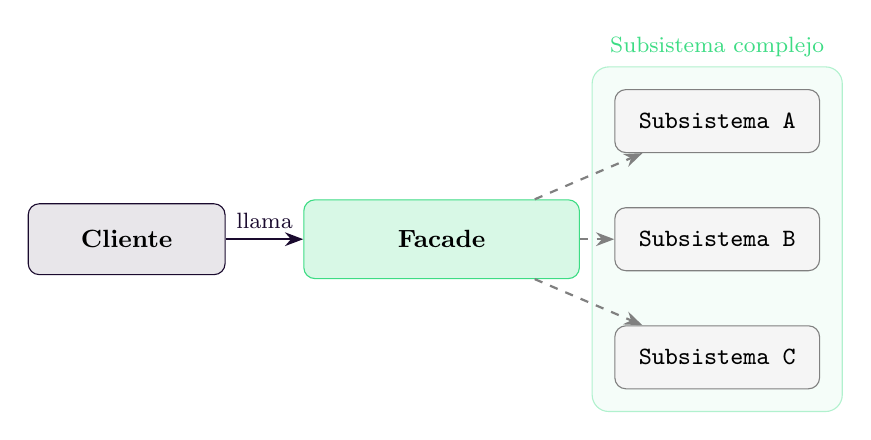
\begin{tikzpicture}[
  client/.style={draw=darkbg,fill=darkbg!10,rounded corners=4pt,
                 minimum width=2.5cm,minimum height=0.9cm,
                 font=\small\bfseries,align=center},
  facade/.style={draw=androidgreen,fill=androidgreen!20,rounded corners=4pt,
                 minimum width=3.5cm,minimum height=1cm,
                 font=\small\bfseries,align=center},
  subsys/.style={draw=gray,fill=lightgray,rounded corners=4pt,
                 minimum width=2.6cm,minimum height=0.8cm,
                 font=\small\ttfamily,align=center},
  arrow/.style={-Stealth,thick},
  darrow/.style={-Stealth,thick,color=gray,dashed}
]
\node[client] (client) at (-4,0) {Cliente};
\node[facade] (facade) at (0,0) {Facade};
\node[subsys] (s1) at (3.5, 1.5)  {Subsistema A};
\node[subsys] (s2) at (3.5, 0)    {Subsistema B};
\node[subsys] (s3) at (3.5,-1.5)  {Subsistema C};

\draw[arrow,color=darkbg] (client) -- node[above,font=\footnotesize]{llama} (facade);
\draw[darrow] (facade) -- (s1);
\draw[darrow] (facade) -- (s2);
\draw[darrow] (facade) -- (s3);

\begin{pgfonlayer}{background}
  \node[draw=androidgreen!40,fill=androidgreen!5,rounded corners=6pt,
        fit=(s1)(s2)(s3),inner sep=8pt,
        label={[font=\footnotesize\color{androidgreen}]above:Subsistema complejo}] {};
\end{pgfonlayer}
\end{tikzpicture}
\end{center}

\subsection{Por que se uso en este proyecto?}

Sin un Facade, cada controlador REST tendría que importar directamente
\texttt{TweetRepository}, \texttt{TweetCommentRepository} y
\texttt{TweetReactionRepository}, y además conocer la lógica de cómo
buscar una carta, validar que existe, crear la entidad relacionada y
guardarla. Eso genera \textbf{acoplamiento fuerte}: si cambia la
lógica de almacenamiento, hay que modificar cada controlador.

Con \texttt{TweetService}, los controladores solo conocen a la fachada
y le delegan todo. La fachada \textit{esconde} la complejidad de
coordinar varios repositorios y concentrar la lógica de negocio.

\subsection{Problema sin Facade vs. solución con Facade}

\begin{warnbox}{Sin Facade: controlador acoplado a múltiples repositorios}
\begin{lstlisting}[language=Java]
// SIN FACADE - el controlador tiene que conocer TODOS los repositorios
@RestController
public class ComentarioController {
    // Acoplado a 3 repositorios directamente
    private final TweetRepository tweetRepo;
    private final TweetCommentRepository comentarioRepo;
    private final TweetReactionRepository reaccionRepo;

    @PostMapping("/{id}/comentarios")
    public ResponseEntity<?> agregar(@PathVariable Long id,
                                     @RequestBody Map<String,String> body) {
        // Logica duplicada en cada controlador
        Tweet tweet = tweetRepo.findById(id)
            .orElseThrow(() -> new RuntimeException("No existe"));
        TweetComment c = new TweetComment(body.get("texto"), tweet);
        comentarioRepo.save(c);
        return ResponseEntity.ok(c);
    }
}
\end{lstlisting}
\end{warnbox}

\begin{patternbox}{Con Facade: controlador simple y lógica centralizada}
\begin{lstlisting}[language=Java]
// CON FACADE - el controlador solo conoce a TweetService
@RestController
public class ComentarioController {
    private final TweetService tweetService; // UNA sola dependencia

    @PostMapping("/{id}/comentarios")
    public ResponseEntity<?> agregar(@PathVariable Long id,
                                     @RequestBody Map<String,String> body) {
        // Solo delega, no sabe como funciona internamente
        TweetComment c = tweetService.addComment(id, body.get("texto"));
        return ResponseEntity.ok(c);
    }
}
\end{lstlisting}
\end{patternbox}

\subsection{Codigo implementado: TweetService}

Esta es la clase central del dominio. Coordina los repositorios
internamente y expone métodos simples y cohesivos:

\begin{filebox}{TweetService.java --- La Fachada}
\begin{lstlisting}[language=Java]
@Service
public class TweetService {

    private final TweetRepository tweetRepository;
    private final TweetCommentRepository tweetCommentRepository;
    private final TweetReactionRepository tweetReactionRepository;
    private final TweetMapperStrategy tweetMapper;

    public TweetService(TweetRepository tweetRepository,
                        TweetCommentRepository tweetCommentRepository,
                        TweetReactionRepository tweetReactionRepository,
                        TweetMapperStrategy tweetMapper) {
        this.tweetRepository = tweetRepository;
        this.tweetCommentRepository = tweetCommentRepository;
        this.tweetReactionRepository = tweetReactionRepository;
        this.tweetMapper = tweetMapper;
    }

    public Page<TweetResponseDTO> getTweets(Pageable pageable) {
        return tweetRepository.findAll(pageable)
                .map(tweetMapper::toResponseDTO);
    }

    public TweetResponseDTO createTweet(Tweet tweet, String username) {
        tweet.setUsername(username);
        Tweet saved = tweetRepository.save(tweet);
        return tweetMapper.toResponseDTO(saved);
    }

    public TweetResponseDTO reactToTweet(Long tweetId, String username,
                                         TweetReactionRequest request) {
        Tweet tweet = tweetRepository.findById(tweetId)
            .orElseThrow(() -> new RuntimeException("Tweet no encontrado"));
        TweetReaction reaction = new TweetReaction(request.getReactionType(),
                                                   username, tweet);
        tweetReactionRepository.save(reaction);
        return tweetMapper.toResponseDTO(tweet);
    }

    public TweetCommentResponseDTO addComment(Long tweetId, String username,
                                              TweetCommentRequest request) {
        Tweet tweet = tweetRepository.findById(tweetId)
            .orElseThrow(() -> new RuntimeException("Tweet no encontrado"));
        TweetComment comment = new TweetComment(request.getContent(),
                                                username, tweet);
        tweetCommentRepository.save(comment);
        return new TweetCommentResponseDTO(
                comment.getId(),
                comment.getContent(),
                comment.getUsername()
        );
    }

    public List<TweetCommentResponseDTO> getComments(Long tweetId) {
        return tweetCommentRepository.findByTweetId(tweetId).stream()
                .map(comment -> new TweetCommentResponseDTO(
                        comment.getId(),
                        comment.getContent(),
                        comment.getUsername()))
                .toList();
    }
}
\end{lstlisting}
\end{filebox}

\subsection{Codigo implementado: Controladores que usan la Facade}

\begin{filebox}{TweetController.java}
\begin{lstlisting}[language=Java]
@CrossOrigin(origins = "*")
@RestController
@RequestMapping("/api/tweets")
public class TweetController {

    private final TweetService tweetService;

    public TweetController(TweetService tweetService) {
        this.tweetService = tweetService;
    }

    @GetMapping("")
    public Page<TweetResponseDTO> getTweet(Pageable pageable) {
        return tweetService.getTweets(pageable);
    }

    @PostMapping("")
    public ResponseEntity<TweetResponseDTO> createTweet(
            @Valid @RequestBody Tweet tweet,
            Authentication authentication) {
        return ResponseEntity.status(201)
                .body(tweetService.createTweet(tweet, authentication.getName()));
    }

    @DeleteMapping("/{id}")
    public ResponseEntity<Void> deleteTweet(
            @PathVariable Long id,
            Authentication authentication) {
        tweetService.deleteTweet(id, authentication.getName());
        return ResponseEntity.noContent().build();
    }
}
\end{lstlisting}
\end{filebox}

\begin{filebox}{TweetCommentController.java}
\begin{lstlisting}[language=Java]
@CrossOrigin(origins = "*")
@RestController
@RequestMapping("/api/tweets")
public class TweetCommentController {

    private final TweetService tweetService;

    public TweetCommentController(TweetService tweetService) {
        this.tweetService = tweetService;
    }

    @GetMapping("/{tweetId}/comments")
    public ResponseEntity<List<TweetCommentResponseDTO>> getComments(
            @PathVariable Long tweetId) {
        return ResponseEntity.ok(tweetService.getComments(tweetId));
    }

    @PostMapping("/{tweetId}/comments")
    public ResponseEntity<TweetCommentResponseDTO> addComment(
            @PathVariable Long tweetId,
            @Valid @RequestBody TweetCommentRequest request,
            Authentication authentication) {

        return ResponseEntity.status(201)
                .body(tweetService.addComment(
                        tweetId,
                        authentication.getName(),
                        request));
    }
}
\end{lstlisting}
\end{filebox}

\begin{filebox}{TweetReactionController.java}
\begin{lstlisting}[language=Java]
@CrossOrigin(origins = "*")
@RestController
@RequestMapping("/api/tweets")
public class TweetReactionController {

    private final TweetService tweetService;

    public TweetReactionController(TweetService tweetService) {
        this.tweetService = tweetService;
    }

    @PostMapping("/{tweetId}/reactions")
    public ResponseEntity<TweetResponseDTO> reactToTweet(
            @PathVariable Long tweetId,
            @Valid @RequestBody TweetReactionRequest request,
            Authentication authentication) {

        return ResponseEntity.ok(
                tweetService.reactToTweet(
                        tweetId,
                        authentication.getName(),
                        request)
        );
    }
}
\end{lstlisting}
\end{filebox}

\subsection{Diagrama UML del patrón Facade en el proyecto}

El siguiente diagrama muestra cómo \texttt{TweetService} actúa como la
única puerta de entrada que los controladores usan para acceder al
subsistema de repositorios y modelos:

\begin{center}
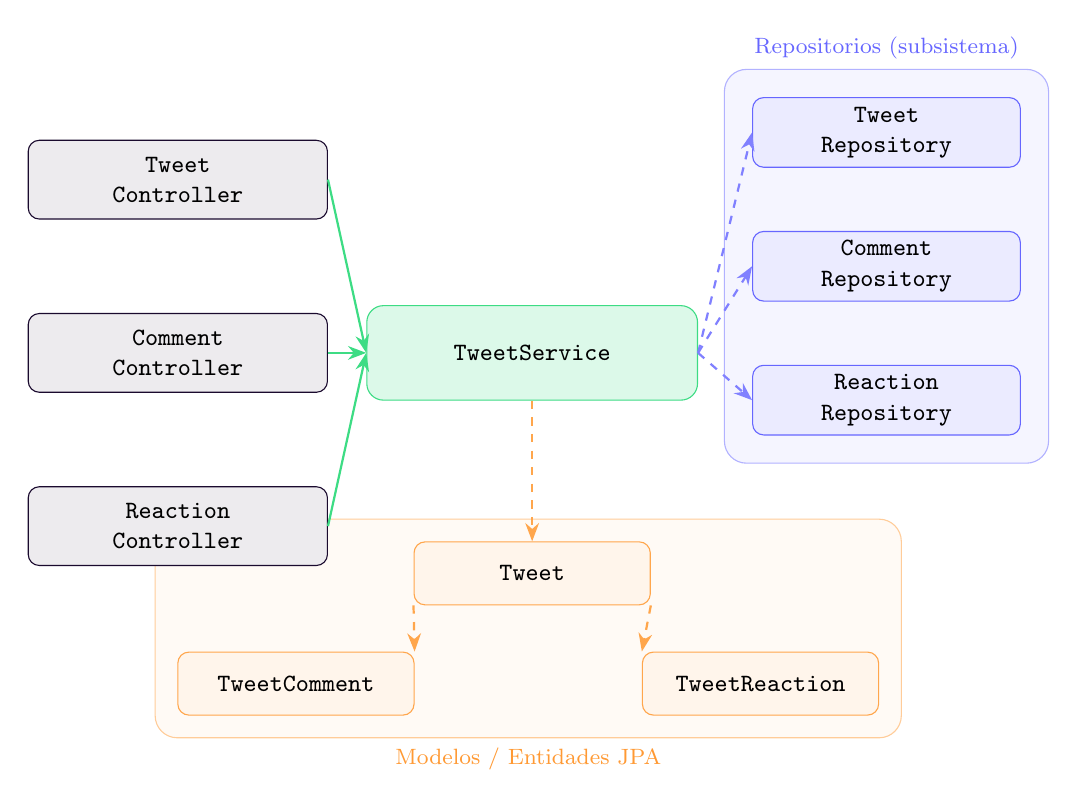
\begin{tikzpicture}[
  ctrl/.style={draw=darkbg,fill=darkbg!8,rounded corners=4pt,
               minimum width=3.8cm,minimum height=1cm,
               font=\small\ttfamily,align=center},
  facade/.style={draw=androidgreen,fill=androidgreen!18,rounded corners=6pt,
                 minimum width=4.2cm,minimum height=1.2cm,
                 font=\small\bfseries\ttfamily,align=center},
  repo/.style={draw=blue!60,fill=blue!8,rounded corners=4pt,
               minimum width=3.4cm,minimum height=0.85cm,
               font=\small\ttfamily,align=center},
  model/.style={draw=orange!70,fill=orange!8,rounded corners=4pt,
                minimum width=3.0cm,minimum height=0.8cm,
                font=\small\ttfamily,align=center},
  arrow/.style={-Stealth,thick,color=androidgreen},
  darrow/.style={-Stealth,thick,color=blue!50,dashed},
  marrow/.style={-Stealth,thick,color=orange!70,dashed}
]

% Controladores (izquierda)
\node[ctrl] (cc) at (0, 2.2)  {Tweet\\Controller};
\node[ctrl] (tc) at (0, 0.0)   {Comment\\Controller};
\node[ctrl] (rc) at (0,-2.2)   {Reaction\\Controller};

% Facade (centro)
\node[facade] (tf) at (4.5, 0) {TweetService};

% Repositorios (derecha arriba)
\node[repo] (tr) at (9, 2.8)  {Tweet\\Repository};
\node[repo] (cr) at (9, 1.1)  {Comment\\Repository};
\node[repo] (rr) at (9,-0.6)  {Reaction\\Repository};

% Modelos (derecha abajo)
\node[model] (tw) at (4.5,-2.8) {Tweet};
\node[model] (cm) at (1.5,-4.2) {TweetComment};
\node[model] (rm) at (7.4,-4.2) {TweetReaction};

% Flechas controladores -> facade
\draw[arrow] (cc.east) -- (tf.west);
\draw[arrow] (tc.east) -- (tf.west);
\draw[arrow] (rc.east) -- (tf.west);

% Flechas facade -> repositorios
\draw[darrow] (tf.east) -- (tr.west);
\draw[darrow] (tf.east) -- (cr.west);
\draw[darrow] (tf.east) -- (rr.west);

% Flechas facade -> modelos
\draw[marrow] (tf.south) -- (tw.north);
\draw[marrow] (tw.south west) -- (cm.north east);
\draw[marrow] (tw.south east) -- (rm.north west);

% Etiqueta subsistema
\begin{pgfonlayer}{background}
  \node[draw=blue!30,fill=blue!4,rounded corners=8pt,
        fit=(tr)(cr)(rr),inner sep=10pt,
        label={[font=\footnotesize\color{blue!60}]above:Repositorios (subsistema)}] {};
  \node[draw=orange!40,fill=orange!4,rounded corners=8pt,
        fit=(tw)(cm)(rm),inner sep=8pt,
        label={[font=\footnotesize\color{orange!80}]below:Modelos / Entidades JPA}] {};
\end{pgfonlayer}

\end{tikzpicture}
\end{center}

\subsection{Beneficios obtenidos del patrón Facade}

\begin{table}[H]
\centering
\renewcommand{\arraystretch}{1.5}
\begin{tabularx}{\textwidth}{>{\bfseries}l X}
\rowcolor{darkbg}
\multicolumn{1}{>{\color{white}\bfseries}l}{Beneficio} &
\multicolumn{1}{>{\color{white}\bfseries}X}{Impacto en el proyecto} \\
\rowcolor{infobg}
Bajo acoplamiento & Los controladores no dependen de los repositorios directamente \\
\rowcolor{white}
Único punto de cambio & Si cambia la lógica de comentarios o reacciones, solo se modifica \texttt{TweetService} \\
\rowcolor{infobg}
Código limpio & Cada controlador queda pequeño y directo \\
\rowcolor{white}
Lógica centralizada & Las reglas del dominio viven en un solo lugar \\
\rowcolor{infobg}
Fácil de testear & Se puede hacer mock de \texttt{TweetService} sin levantar repositorios \\
\end{tabularx}
\caption{Beneficios del patrón Facade en el proyecto}
\end{table}

%=============================================================
\section{Patron Repository}
%=============================================================

\begin{patternbox}{¿Qué es el patrón Repository?}
El Repository actúa como una colección de objetos en memoria. En lugar
de escribir SQL directamente en la lógica de negocio, se crea una
interfaz que define qué operaciones se pueden hacer con cada entidad.
Spring Data JPA genera automáticamente la implementación a partir
del nombre de los métodos, sin necesidad de escribir SQL.
\end{patternbox}

\subsubsection{Repositorios implementados}

\begin{filebox}{TweetRepository.java}
\begin{lstlisting}[language=Java]
@Repository
public interface TweetRepository
        extends JpaRepository<Tweet, Long> {

    Page<Tweet> findAll(Pageable pageable);
}
\end{lstlisting}
\end{filebox}

\begin{filebox}{TweetCommentRepository.java}
\begin{lstlisting}[language=Java]
@Repository
public interface TweetCommentRepository
        extends JpaRepository<TweetComment, Long> {

    List<TweetComment> findByTweetId(Long tweetId);
}
\end{lstlisting}
\end{filebox}

\begin{filebox}{TweetReactionRepository.java}
\begin{lstlisting}[language=Java]
@Repository
public interface TweetReactionRepository
        extends JpaRepository<TweetReaction, Long> {

    List<TweetReaction> findByTweetId(Long tweetId);
    long countByTweetId(Long tweetId);
}
\end{lstlisting}
\end{filebox}

\begin{filebox}{UserRepository.java}
\begin{lstlisting}[language=Java]
@Repository
public interface UserRepository
        extends JpaRepository<User, Long> {

    Optional<User> findByUsername(String username);

    boolean existsByUsername(String username);

    boolean existsByEmail(String email);
}
\end{lstlisting}
\end{filebox}

%=============================================================
\section{Modelos / Entidades JPA}
%=============================================================

Los modelos son clases Java anotadas con \texttt{@Entity} que Hibernate
mapea automáticamente a tablas de PostgreSQL.

\begin{filebox}{Tweet.java --- Entidad principal}
\begin{lstlisting}[language=Java]
@Entity
@Table(name = "tweets")
public class Tweet {

    @Id
    @GeneratedValue(strategy = GenerationType.IDENTITY)
    private Long id;

    private String nombre;

    private String rareza;

    private Integer costoElixir;

    @Column(length = 1000)
    private String urlImagen;

    private String username;
}
\end{lstlisting}
\end{filebox}

\begin{filebox}{TweetComment.java}
\begin{lstlisting}[language=Java]
@Entity
@Table(name = "tweet_comments")
public class TweetComment {

    @Id
    @GeneratedValue(strategy = GenerationType.IDENTITY)
    private Long id;

    private String content;

    private String username;

    @ManyToOne(fetch = FetchType.LAZY)
    @JoinColumn(name = "tweet_id")
    @JsonIgnore
    private Tweet tweet;
}
\end{lstlisting}
\end{filebox}

\begin{filebox}{TweetReaction.java}
\begin{lstlisting}[language=Java]
@Entity
@Table(name = "tweet_reactions")
public class TweetReaction {

    @Id
    @GeneratedValue(strategy = GenerationType.IDENTITY)
    private Long id;

    private String reactionType;

    private String username;

    @ManyToOne(fetch = FetchType.LAZY)
    @JoinColumn(name = "tweet_id")
    @JsonIgnore
    private Tweet tweet;
}
\end{lstlisting}
\end{filebox}

\begin{filebox}{User.java}
\begin{lstlisting}[language=Java]
@Entity
@Table(name = "users")
public class User {

    @Id
    @GeneratedValue(strategy = GenerationType.IDENTITY)
    private Long id;

    @NotBlank
    private String username;

    @NotBlank
    @Column(unique = true)
    private String email;

    @NotBlank
    private String password;
}
\end{lstlisting}
\end{filebox}

%=============================================================
\section{Patron MVC}
%=============================================================

\begin{patternbox}{¿Qué es el patrón MVC?}
MVC divide la aplicación en tres capas: el \textbf{Modelo} maneja
los datos, la \textbf{Vista} muestra la interfaz al usuario, y el
\textbf{Controlador} recibe las peticiones y coordina entre los otros
dos. Esto permite cambiar la interfaz sin tocar la lógica del negocio.
\end{patternbox}

En este proyecto MVC se aplica en dos niveles simultáneos:

\begin{itemize}
  \item \textbf{Backend (Spring Boot):} las entidades JPA son el Modelo,
        los \texttt{@RestController} son los Controladores, y el JSON
        que retorna la API es la representación de la Vista.
  \item \textbf{Frontend (Flutter):} los widgets de Flutter son la Vista
        que consume la API y muestra los datos al usuario.
\end{itemize}

%=============================================================
\section{Patron DTO}
%=============================================================

\begin{patternbox}{¿Qué es un DTO?}
DTO significa \textit{Data Transfer Object}. Se utiliza para transferir
únicamente la información necesaria entre backend y frontend sin exponer
directamente las entidades internas de la base de datos.
\end{patternbox}

\subsection{Aplicación en el proyecto}

El sistema utiliza DTOs para respuestas y peticiones, lo que permite
controlar exactamente qué campos viajan por la API.

\begin{filebox}{TweetResponseDTO.java}
\begin{lstlisting}[language=Java]
public class TweetResponseDTO {

    private Long id;
    private String nombre;
    private Integer costoElixir;
    private String rareza;
    private String urlImagen;
    private String username;
}
\end{lstlisting}
\end{filebox}

\begin{filebox}{TweetCommentResponseDTO.java}
\begin{lstlisting}[language=Java]
public class TweetCommentResponseDTO {

    private Long id;
    private String content;
    private String username;
}
\end{lstlisting}
\end{filebox}

\begin{filebox}{TweetReactionRequest.java}
\begin{lstlisting}[language=Java]
public class TweetReactionRequest {

    private String reactionType;
}
\end{lstlisting}
\end{filebox}

%=============================================================
\section{Patron Dependency Injection}
%=============================================================

\begin{patternbox}{¿Qué es Dependency Injection?}
Dependency Injection permite que Spring inyecte dependencias
automáticamente mediante el constructor. Esto reduce el acoplamiento
entre clases y facilita el mantenimiento y las pruebas.
\end{patternbox}

\subsection{Aplicación en el proyecto}

Todos los controladores y servicios utilizan inyección de dependencias.

\begin{filebox}{AuthController.java}
\begin{lstlisting}[language=Java]
@RestController
@RequestMapping("/api/auth")
public class AuthController {

    private final AuthService authService;

    public AuthController(AuthService authService) {
        this.authService = authService;
    }
}
\end{lstlisting}
\end{filebox}

\begin{filebox}{TweetController.java}
\begin{lstlisting}[language=Java]
private final TweetService tweetService;

public TweetController(TweetService tweetService) {
    this.tweetService = tweetService;
}
\end{lstlisting}
\end{filebox}

\subsection{Beneficio}
La lógica queda desacoplada y se pueden cambiar implementaciones sin modificar el resto de las clases.

%=============================================================
\section{Patron Singleton}
%=============================================================

\begin{patternbox}{¿Qué es Singleton?}
Singleton garantiza que una clase tenga una única instancia compartida
durante toda la ejecución de la aplicación.
\end{patternbox}

\subsection{Aplicación en el proyecto}

Spring maneja los beans como Singleton por defecto.  
En particular, los servicios, controladores y repositorios se crean una sola vez
y se reutilizan durante toda la ejecución.

\begin{filebox}{TweetService.java}
\begin{lstlisting}[language=Java]
@Service
public class TweetService {
}
\end{lstlisting}
\end{filebox}

\subsection{Beneficio}
Evita crear objetos innecesarios y mantiene una instancia compartida de los componentes principales.

%=============================================================
\section{Patron Strategy}
%=============================================================

\begin{patternbox}{¿Qué es Strategy?}
Strategy permite intercambiar algoritmos o reglas de comportamiento
sin modificar al cliente que los usa.
\end{patternbox}

\subsection{Aplicación en el proyecto}

Spring Security utiliza distintas estrategias internas para autenticación
y autorización mediante JWT y roles.

\begin{filebox}{TestController.java}
\begin{lstlisting}[language=Java]
@GetMapping("/admin")
@PreAuthorize("hasRole('ADMIN')")
public String adminAccess() {
    return "Clash Royale admin board.";
}
\end{lstlisting}
\end{filebox}

Cada ruta aplica una estrategia diferente de autorización según el rol del usuario.

%=============================================================
\section{Patron Builder}
%=============================================================

\begin{patternbox}{¿Qué es Builder?}
Builder facilita la construcción de objetos complejos paso a paso
y mejora la legibilidad del código.
\end{patternbox}

\subsection{Aplicación en el proyecto}

Spring usa un estilo fluido en la construcción de respuestas HTTP
con \texttt{ResponseEntity}.

\begin{filebox}{ResponseEntity}
\begin{lstlisting}[language=Java]
return ResponseEntity.status(201)
        .body(tweetService.createTweet(tweet, authentication.getName()));
\end{lstlisting}
\end{filebox}

\begin{lstlisting}[language=Java]
return ResponseEntity.noContent().build();
\end{lstlisting}

\subsection{Beneficio}
El código queda más expresivo y se entiende con claridad el tipo de respuesta que se está construyendo.

%=============================================================
\section{Patron Proxy}
%=============================================================

\begin{patternbox}{¿Qué es Proxy?}
Proxy controla el acceso a otro objeto y puede aplicar validaciones
o filtros antes de ejecutar la lógica real.
\end{patternbox}

\subsection{Aplicación en el proyecto}

Spring Security actúa como proxy antes de permitir acceso a endpoints protegidos,
interceptando peticiones y verificando el token JWT y los roles.

\begin{filebox}{TestController.java}
\begin{lstlisting}[language=Java]
@PreAuthorize("hasRole('ADMIN')")
public String adminAccess() {
    return "Clash Royale admin board.";
}
\end{lstlisting}
\end{filebox}

Spring intercepta la petición antes de ejecutar el método real.

%=============================================================
\section{Endpoints de la API REST}
%=============================================================

\begin{table}[H]
\centering
\renewcommand{\arraystretch}{1.4}
\begin{tabularx}{\textwidth}{>{\ttfamily\footnotesize}l
                              >{\ttfamily\footnotesize}l X}
\rowcolor{darkbg}
\multicolumn{1}{>{\color{white}\bfseries\rmfamily\small}l}{Metodo} &
\multicolumn{1}{>{\color{white}\bfseries\rmfamily\small}l}{Ruta} &
\multicolumn{1}{>{\color{white}\bfseries\rmfamily\small}X}{Descripcion} \\
\rowcolor{androidgreen!15}
\multicolumn{3}{l}{\textbf{\small Autenticación}} \\
POST   & /api/auth/signin   & Iniciar sesión \\
\rowcolor{lightgray}
POST   & /api/auth/signup   & Registrar usuario \\
\rowcolor{androidgreen!15}
\multicolumn{3}{l}{\textbf{\small Tweets / Cartas}} \\
\rowcolor{lightgray}
GET    & /api/tweets        & Listar publicaciones paginadas \\
POST   & /api/tweets        & Crear nueva publicación \\
\rowcolor{lightgray}
DELETE & /api/tweets/\{id\} & Eliminar publicación \\
\rowcolor{androidgreen!15}
\multicolumn{3}{l}{\textbf{\small Reacciones y comentarios}} \\
\rowcolor{lightgray}
POST   & /api/tweets/\{id\}/reactions   & Agregar reacción \\
GET    & /api/tweets/\{id\}/comments     & Lista de comentarios \\
\rowcolor{lightgray}
POST   & /api/tweets/\{id\}/comments     & Agregar comentario \\
\end{tabularx}
\caption{Endpoints principales de la API REST}
\end{table}

%=============================================================
\section{Arquitectura y Despliegue}
%=============================================================

\begin{center}
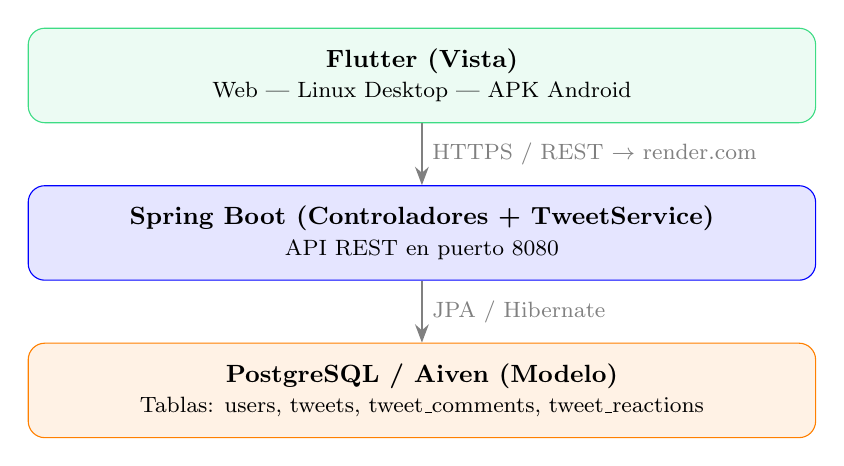
\begin{tikzpicture}[
  layer/.style={draw=#1,fill=#1!10,rounded corners=6pt,
                minimum width=10cm,minimum height=1.2cm,
                font=\small\bfseries,align=center},
  arrow/.style={-Stealth,thick,color=gray}
]
\node[layer=androidgreen] (flutter) at (0,4)
  {Flutter (Vista)\\
   \footnotesize\normalfont Web --- Linux Desktop --- APK Android};
\node[layer=blue] (spring) at (0,2)
  {Spring Boot (Controladores + TweetService)\\
   \footnotesize\normalfont API REST en puerto 8080};
\node[layer=orange] (db) at (0,0)
  {PostgreSQL / Aiven (Modelo)\\
   \footnotesize\normalfont Tablas: users, tweets, tweet\_comments, tweet\_reactions};
\draw[arrow] (flutter) -- node[right,font=\footnotesize]{HTTPS / REST $\rightarrow$ render.com} (spring);
\draw[arrow] (spring) -- node[right,font=\footnotesize]{JPA / Hibernate} (db);
\end{tikzpicture}
\end{center}

\vspace{0.5em}

El backend se empaqueta con Maven en un JAR y se contenedorizó con Docker.
Las variables de entorno \texttt{DATABASE\_URL}, \texttt{DB\_USER} y
\texttt{DB\_PASSWORD} configuran la conexión a Aiven desde Render.

\begin{tcolorbox}[
  enhanced, colback=darkbg, colframe=androidgreen,
  arc=4pt, boxrule=1pt,
  left=10pt, right=10pt, top=8pt, bottom=8pt,
]
\color{androidgreen}\ttfamily\small
\# Desarrollo local\\
\$ mvn spring-boot:run -Dspring-boot.run.profiles=local\\[4pt]
\# Producción (Render ejecuta el backend con Docker)\\
\$ flutter build web --release \quad\# frontend web\\
\$ flutter build apk --release \quad\# APK Android
\end{tcolorbox}

%=============================================================
\section{Conclusion}
%=============================================================

El patrón \textbf{Facade} fue el aporte estructural más importante del
proyecto. Al encapsular toda la coordinación entre \texttt{TweetRepository},
\texttt{TweetCommentRepository} y \texttt{TweetReactionRepository} dentro de
\texttt{TweetService}, se logró que los controladores REST quedaran con
una sola dependencia y con una estructura mucho más limpia. Eso hace
el sistema más fácil de mantener: si la lógica de comentarios o reacciones
cambia, solo se modifica la fachada.

Los \textbf{repositorios} eliminaron la necesidad de escribir SQL, ya que
Spring Data JPA genera las consultas automáticamente a partir del nombre
de los métodos como \texttt{findByTweetId} o \texttt{existsByUsername}.

El patrón \textbf{MVC} permitió desarrollar el backend (Spring Boot) y
el frontend (Flutter) de forma completamente independiente, comunicándose
únicamente a través de la API REST desplegada en Render.

\end{document}